\documentclass[11pt,a4paper]{report}
\usepackage{marvosym}

\assignment{3}
\group{...}
\students{..........}{..........}

\begin{document}

\maketitle

Answer to the questions by by adding text in the boxes. Do not modify anything else in the template.  The size of the boxes indicate the place you \textit{can} use, but you \textit{need not} use all of it (it is not an indication of any expected length of answer). Be as concise as possible! A good short answer is better than a lot of nonsense ;-)
\bigskip

\section{Alpha-Beta search (5~pts)}

Answer questions 1 to 4 by inserting an image of the tree in the corresponding box. This may either be an edited version of \texttt{minimax.pdf} or \texttt{minimax.png} (using paint, gimp, etc.), or a photograph of a drawing you made by hand. In any case, the images must be \textbf{clear} in order to be graded.

\begin{enumerate}
\item Perform the MiniMax algorithm on the following tree, i.e.
      put a value to each node. Circle the move the root player should do. \textbf{(1~pt)}
\end{enumerate}

\begin{answers}[8cm]
%TODO Insert the path to your image between the {}
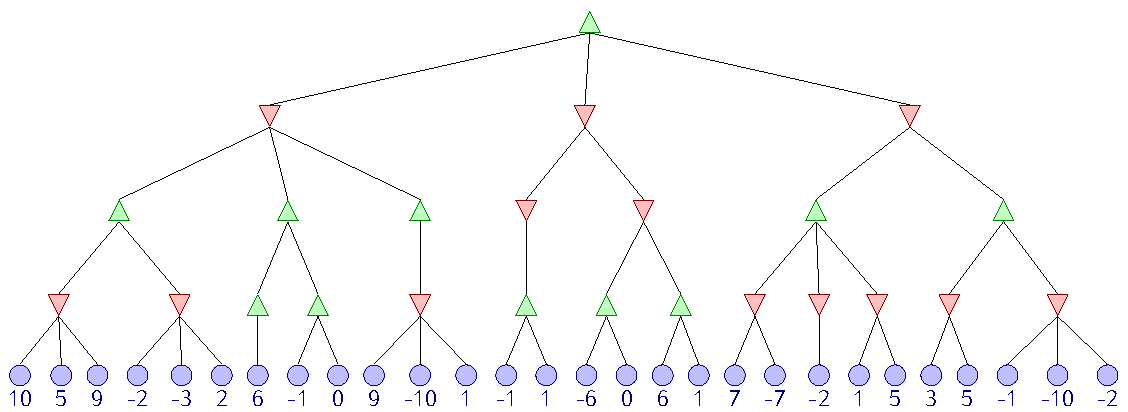
\includegraphics[scale=.85]{minimax.pdf}
\end{answers}




\clearpage
\begin{enumerate}
\item[2.] Perform the Alpha-Beta algorithm on the same tree.
      At each non terminal node, put the successive values of $\alpha$ and
      $\beta$. Cross out the arcs reaching non visited nodes. Assume a
      left-to-right node expansion. \textbf{(1~pt)}
\end{enumerate}

\begin{answers}[8cm]
%TODO Insert the path to your image between the {}
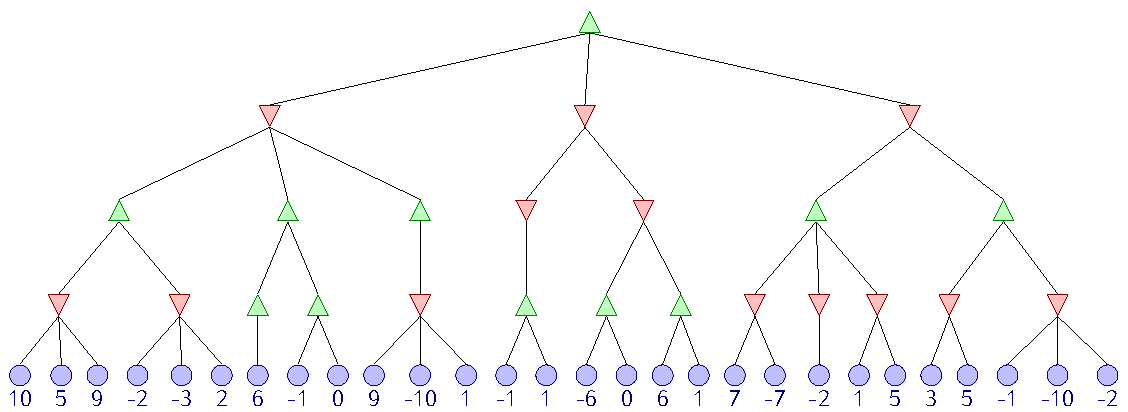
\includegraphics[scale=.85]{minimax.pdf}
\end{answers}





\begin{enumerate}
\item[3.] Do the same, assuming a right-to-left node expansion instead.  \textbf{(1~pt)}
\end{enumerate}

\begin{answers}[8cm]
%TODO Insert the path to your image between the {}
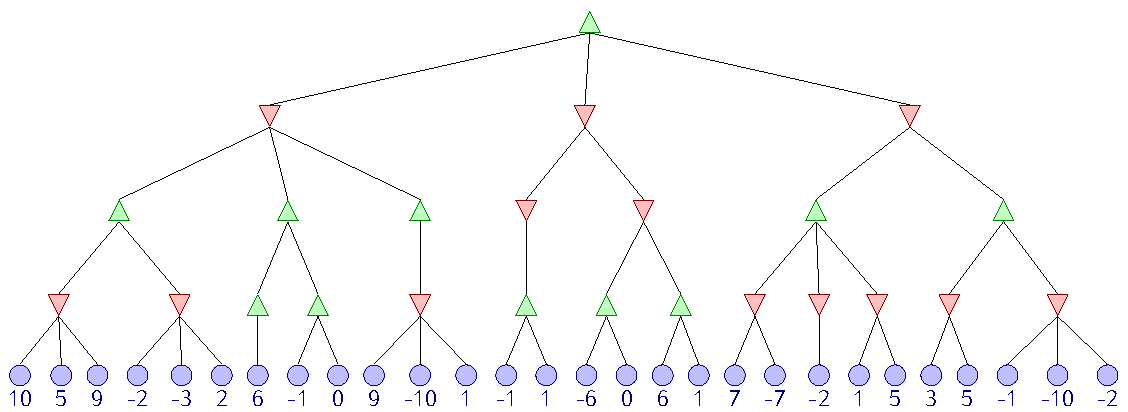
\includegraphics[scale=.85]{minimax.pdf}
\end{answers}




\clearpage
\begin{enumerate}
\item[4.] Can the nodes be ordered in such a way that Alpha-Beta pruning can cut off
      more branches (in a left-to-right node expansion)? If no, explain why; if
      yes, give the new ordering and the resulting new pruning. \textbf{(1~pt)}
\end{enumerate}

\begin{answers}[8cm]
%TODO Insert the path to your image between the {}
%\includegraphics[scale=.85]{...}
\end{answers}




\begin{enumerate}
\item[5.] How does Alpha-Beta need to be modified for games with more than two players? \textbf{(1~pt)}
\end{enumerate}

\begin{answers}[11cm]
%TODO Insert your answer here
\end{answers}





\clearpage
\section{Seega (35~pts)}
\medskip

\subsection{A Basic Alpha-Beta Agent (5~pts on INGInious; nothing to report)}
\medskip


\subsection{Evaluation function (5~pts)}

\begin{enumerate}
\item[5.] What are the weak points of the evaluation functions of your basic agent? \textbf{(2~pts)}
\end{enumerate}

\begin{answers}[19cm]
%TODO Insert your answer here
\end{answers}


\clearpage
\begin{enumerate}
\item[6.] As described in the class, an evaluation function is often a linear combination of
some features. Describe new features of a state that can be interesting when evaluating a state of this game. \textbf{(2~pts)}
\end{enumerate}

\begin{answers}[20cm]
%TODO Insert your answer here
\end{answers}



\clearpage
\begin{enumerate}
\item[7.] Describe precisely your improved evaluation function. \textbf{(1~pt)}
\end{enumerate}

\begin{answers}[20cm]
%TODO Insert your answer here
\end{answers}






\clearpage
\subsection{Successors function (4~pts)}

\begin{enumerate}
\item[8.] Give an upper bound on the maximum number of actions that can be performed in
any given state. If you can't, explain how you could estimate what is the average
number of successors and estimate it. \textbf{(1~pt)}
\end{enumerate}

\begin{answers}[9cm]
%TODO Insert your answer here
\end{answers}






\begin{enumerate}
\item[9.] What do you loose by ignoring some of the successors? \textbf{(1~pt)}
\end{enumerate}

\begin{answers}[9cm]
%TODO Insert your answer here
\end{answers}






\begin{enumerate}
\item[10.] Could reordering the successors help the performance of your agent? If so, in what order should the successors be returned in order to help Alpha-Beta
prune the search tree? \textbf{(1~pt)}
\end{enumerate}

\begin{answers}[9cm]
%TODO Insert your answer here
\end{answers}





\begin{enumerate}
\item[11.] Describe you successor function. \textbf{(1~pt)}
\end{enumerate}

\begin{answers}[9cm]
%TODO Insert your answer here
\end{answers}





\clearpage
\subsection{Cut-off function (4~pts)}


\begin{enumerate}
\item[12.] The \lstinline|cutoff| method receives an argument called
    \lstinline|depth|. Explain precisely what is called the
    \emph{depth} in the \lstinline|minimax.py| implementation. \textbf{(1~pt)}
\end{enumerate}

\begin{answers}[6cm]
%TODO Insert your answer here
\end{answers}





\begin{enumerate}
\item[13.] The \lstinline|cutoff| function is also the one responsible for identifying which states lead to the end of the game (and so possible victory or defeat). One such situation is a draw, called a \lstinline|boring| state in the implementation, where each player has managed to build a ``barrier'' behind which pawns can move indefinitely without risking to be attacked. In the implementation, this is dealt with by ending the game when 50 boring moves have occurred. Why could such an approach be problematic for an Alpha-Beta agent? How could you remedy this? \textbf{(1~pt)}
\end{enumerate}

\begin{answers}[10cm]
%TODO Insert your answer here
\end{answers}





\begin{enumerate}
\item[14.] In the Seega contest your agent will be credited a limited time.
How do you manage that time? How can you make sure that you will never timeout?
Explain how you can use \emph{iterative deepening} to avoid timeouts. \textbf{(1~pt)}
\end{enumerate}

\begin{answers}[10cm]
%TODO Insert your answer here
\end{answers}






\begin{enumerate}
\item[15.] Describe your cut-off function. \textbf{(1~pt)}
\end{enumerate}

\begin{answers}[9cm]
%TODO Insert your answer here
\end{answers}





\clearpage
\subsection{A Smart Alpha-Beta Agent (6~pts on INGInious)}
\medskip

\subsection{Contest (6~pts on INGInious; 5~pts for report)}


\begin{enumerate}
\item[18.] Describe concisely your super tough agent. \textbf{(5~pts)}
\end{enumerate}

\begin{answers}[20cm]
%TODO Insert your answer here and in the following frame if needed
\end{answers}

\begin{answers}[23cm]
%TODO Continue your answer here
\end{answers}





\end{document}
